% A Preliminary Literature Review which indicates: 
% (i) that you have studied the work of the major authors in your research field 
% (ii) that you are familiar with the major themes relevant to that subject area 
% (iii) what further investigations you intend to pursue as part of this dissertation. 
% You should bear in mind that you are reviewing the literature in order to develop sharper, 
% more insightful and focused research questions about your topic. 
% Therefore, your literature review should lead to and justify your research objectives and questions.

\xchapter{Fundamentação teórica}
{Este capítulo apresenta conceitos necessários para a compreensão do trabalho.}
\label{fundamentacao}

%À medida que os softwares se tornam uma tecnologia generalizada em praticamente
%todos os aspectos da condição humana, também são inseridos firmemente no meio
%acadêmico, softwares analisam dados, simulam o mundo real, e visualizam
%resultados.

\section{Ecossistema de software}

% ecossistema pode estar organizado em relacões de benefício mútuo

Ecossistema de software é definido, segundo \citeonline{manikas2013software},
como a interação entre diversos atores numa plataforma tecnológica comum
resultando em novas soluções de softwares ou novos serviços. Cada ator neste
sistema é motivado por um conjunto de interesses e conectam-se entre si e ao
próprio sistema numa relação simbiótica, fazendo a plataforma tecnológica
evoluir enquanto permite o envolvimento e contribuição de novos e diferentes
atores.

O relacionamento entre os atores neste ecossistema possibilita benefícios
mútuos para ambos os lados, os tipos de benefícios podem variar enormemente
dependendo do ator e da natureza do ecosistema, num ecossistema comercial por
exemplo, os atores ganham receita financeira diretamente, enquanto num sistema
não-comercial os atores estão motivados por questões não-monetários (fama,
conhecimento, ideologia, etc).

Neste tipo de relacionamento todos são beneficiados, os atores e o próprio
ecossistema, os benefícios dos atores aumentam com o crescimento do ecossistema
e os benefícios do ecossistema aumentam pelas atividades dos seus atores,
o ecosistema de software possibilita esse tipo relação simbiótica apesar de
não determinar que todo ecossistema aproveite tal benefício.

%Adicionalmente as relacões entre os atores do ecosistema como um todo
%são de mútuo interesse (mutualismo):
%
%O relacionamento entre os atores em um ecossistema de software, por outro lado,
%são caracterizados pela alto espectro de relacionamentos simbioticos.
%
%Dependendo dos atores e suas atividades, dois atores podem ter benefícios
%mútuos (mutualismo), estar em competição direta (competition/antagonism),
%estarem não afetados (neutralism) ou um não afetado enquanto o outro é
%beneficiado (amensalism) ou prejudicado (parasitism) por seu relacionamento

\section{Ecossistema de software acadêmico}

O ecossistema de software acadêmico possui a particularidade de estar inserido
num contexto que se relaciona com a economia de reputação científica,
especialmente com o sistema de publicação, sendo influenciado e influenciando
o impacto de suas publicações.

\citeonline{howison2015understanding} criou um framework para pensar e refletir
sobre o ecossistema de software, a Figura
\ref{process-model-scientific-software} apresenta um modelo simplificado do
processo de software na ciência, usuário final, produtores e distribuidores,
administradores de infraestrutura e pesquisadores preocupados com o
funcionamento do ecossistema.

\begin{figure}[h]
  \center
  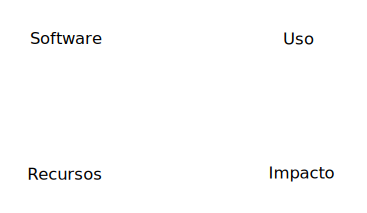
\includegraphics[scale=0.5]{imagens/process-model-scientific-software.png}
  \caption{A process model of software in science \cite{howison2015understanding}}
  \label{process-model-scientific-software}
\end{figure}

%Unlike other technologies supporting science, software can
%be copied and distributed at essentially no cost, potentially
%opening the door to unprecedented levels of sharing and col-
%laborative innovation. \cite{howison2011scientific}
%
%While some of these seem relatively unproblematic, such as commercial
%production in fields with immediately valuable applications, others appear
%problematic. In particular we highlighted the potentially pernicious
%implications of the academic credit production system for collaboration and
%maintenance.

\subsection{Usuário final}

Cientistas engajado em domínio da ciência ocupam papel chave no ecosistema de
software acadêmico, estão dirigindo suas pesquisas e investigações, e no
processo juntaram artefatos de software para coletar, gerenciar, formatar,
analisar, modelar e visualizar dados, com o objetivo final de publicar seus
resultados na literatura acadêmica.

Estão preocupados com disponibilidade, qualidade e usabilidade dos softwares,
também com a capacidade de continuar úteis cientificamente, e poderão continuar
serem utilizados em conjunto com outros softwares.

Estes usuários estão interessados em saber o que os outros cientistas estão
usando, softwares com alta adoção no domínio mantém os pesquisadores mais
focados em suas contribuições científicas, uma vez que os revisores tem alta
chance de entenderem o método utilizado.

Finalmente softwares muito utilizados e adotados são tanto sinal de sua qualidade
quanto a garantia que a equipe, estudantes e colaboradores conseguirão encontrar
e possivelmente encontrar ajuda entre outros peers para resolver questões sobre o
software, liberando assim para terem foco na pesquisa.

\subsection{Produtor de software}

Um segundo papel é o que produtor de softwares acadêmicos, e distribuição. Varia
de indivíduos a times, ambos chamado de projetos para facilidade, produzindo
artefatos que são usados por pequenos grupos ou disciplinas inteiras.

Alguns softwares são desenvolvidos e muitas vezes ficam confinados em seus laboratórios
ou grupos, mas eventualmente são compartilhados e potencialmente amplamente adotados, tornando
o cientista parte do ecosistema do software (Van de Geijin 1997).

Muitas vezes são desenvolvidos em colaborações próximas entre cientistas de computação e
outras áreas, eles desenvolvem algoritmos que refletem as pesquisas dos pesquisadores
do domínio em questão. Um desafio é abstrair os problemas e implementar soluções que
podem ser adotadas por outros cientistas, especialmente em outros domínios.

Projetos se preocupam com o impacto cientifico tanto em termos de numero quando
tipo de usuários seu software atinge, e como seus softwares contribuem para a
ciencia que outros estão realizando.

Alguns projetos são gerenciados no estilo de código aberto, e tem
atraido com sucesso contribuições de muitos cientistas, incluindo
uma calda longa de contriuição que tem feito pequenas mas substanciais
contribuições.

\subsection{Provedor de infraestrutura}

Um terceiro papel é quem provê um cojunto de softwares que são
disponíveis aos usuários finais em seus trabalhos de pesquisa.
Este papel pode ser desempenhado como ciberinfraestrutura de software
em centros de supercomputação através de provedores de computação
em nuvem ou podem ser distribuidos, podem ser disponiveis para usuarios
fazer download em seus computadores pessoais.

Do ponto de vista de ecosistema, ambos os tipos de distribuiça
estão interessados nas mesmas questões: quem usa, ou não usa?
Qual versão usa? Em qual frequencia atualiza?

\subsection{Pesquisador}

Um último papel é daqueles preocupados sobre o funcionamento do
próprio ecosistema e sua contribuição para a ciência.

Costuma ser agencias de financiamento mas pode ser também cientistas sênior do
domínio que refletem além de seu trabalho individual e pensam em seus campos
como um todo.

As preocupações rondam ao redor de questões sobre operação do ecosistema como
um sistema que toma recursos (tempo, dinheiro e atenção) e afeta a conduta da
ciência, tanto o geral como em campos individuais, complementado pelo interesse
de saber como o comportamento desse sistema pode ser influenciado.

%Essas preocupações gerais sugerem um conjunto de questões específicas, com foco
%em padrões globais e padrões emergentes dentro do ecossistema, incluindo: Quais
%recursos foram destinados à produção de software? Quantos usuários ou
%comunidades de usuários têm projetos? Quais são os impactos científicos desse
%uso? Os números de usuários crescem? Os projetos possuem recursos e habilidades
%suficientes para gerenciar seu crescimento? Quais projetos possuem
%funcionalidades sobrepostas? Há quanto tempo os pedaços de software e projetos
%persistem? Nós desconectamos as comunidades de usuários e desenvolvedores? São
%componentes específicos, ou camadas de componentes, faltam? Que código
%geralmente é usado em conjunto; são os projetos e as pessoas que produzem esses
%componentes se comunicando adequadamente? Como podemos sustentar o software
%crítico?

Junto com estas questões estão as questões de como influenciar o ecossistema,
incluindo questões de pontos de inflexão que levam ao uso coalescente, bem como
a intervenções políticas diretas incentivando o uso de componentes específicos.

%Aqui há uma clara tensão entre um desejo de flexibilidade e liberdade, ligado
%às expectativas de inovação científica e desejos de estruturas de autoridade e
%controle de coordenação. As questões de influência incluem: como os programas
%de financiamento e quais os requisitos em suas chamadas, resultaram em software
%amplamente utilizado e impacto científico substancial? Quais são as
%características dos campos que alcançaram maior coalescência? Quais jornais e
%conferências têm políticas exemplares? Como o trabalho de software é visto
%dentro das práticas de contratação e avaliação, como os casos de posse?
%
%\cite{howison2015understanding}

\section{Modelo de produção de software acadêmico}

% recurso, uso e impacto

Estes atores participam do ecossistema dentro de seus próprios interesses, mas
sempre causando um impacto de volta no sistema, os usuários finais cientistas
(diretamente ou indiretamente) usam softwares acadêmicos para fazer ciência,
resultando em impacto científico, este impacto científico então justifica
investimento de novos recursos, que faz o ecossistema crescer fazendo os softwares
existentes evoluirem ou criando novos softwares.

%seja para fins de planejamento ou reflexão
%seja como retrospectiva para avaliar investimentos realizados.
%
%Recursos são devotados para a produção de software acadêmico. Usuários finais
%cientistas (diretamente ou indiretamente) usam softwares acadêmicos para fazer
%ciência, resultando em impacto científico. Impacto científico então justifica
%investimentos e recursos, seja de forma antecipada para fins de planejamento,
%seja como retrospectiva para avaliar investimentos realizados.

Compreender como os softwares acadêmicos vem a ser criados é um primeiro
passo crucial para avaliar seu .... quem faz, o quê, e quando?

\subsection{Recursos}

Cinco modelos de produção de software na ciência, distinguidos principalmente
pela motivação principal: (1) ganho monetário direto (comercial software,
employed software developers), (2) reputação acadêmica (incidental software,
dirigido pela necessidade científica direta), (3) prática de software paralela
(scientific needed enhanced by publishing 'software papers' alongside domain research),
(4) um software de uma subárea de pesquisa (reputação direta pelo trabalho do software),
(5) híbridos como licença-dual e 'software work' dentro de grandes colaborações
(software como uma contribuição científica direta).

Os recursos investidos na produção de software acadêmico vem de diversas
fontes, incluem ganhos monetários diretos, recurso alocado em projetos,
colaboração em 'service work', e ostensivamente 'tempo livre' dos pesquisadores
em busca de soluções em suas pesquisas, que perpassa financiamentos diversos,
carreira individual do cientista, estudantes de graduação, prêmios, etc.

O desenvolvimento de software acadêmico, assim como de qualquer outro
software, exige conhecimento sobre o domínio de aplicação, o que torna o
seu desenvolvimento essencialmente diferente é que este conhecimento pode ser,
por exemplo, entender como o DNA genômico se transforma em cristais de
proteína, ou os meandros da dinâmica dos fluidos, ou como resolver 20 equações
diferenciais parciais simultâneas \cite{segal2008developing}.

Isto faz com que os próprios cientistas acabem desenvolvendo os seus softwares,
um estudo entre cientistas do reino unido mostrou, por exemplo, que 56\%
desenvolvem seus próprios softwares, pelo menos pacialmente
\cite{hettrick_2014_14809}, outro estudo similar mostrou que na astronomia este
número chega a 90\% \cite{momcheva2015software}.

\subsection{Uso}

% ... software é distribuido, utilizado e dá suporte à ciencia, gerando impacto ...

Software acadêmico ({\it academic software}) é todo software usado para
coletar, processar ou analisar resultados de pesquisas com intenção de ser
publicados na literatura academica (seja num jornal, revista, conferência,
monografia, livro ou tese), podem ser desde protótipos escritos pelos próprios
cientistas, até mesmo produtos completos desenvolvidos profissionalmente
\cite{allen2017engineering}.

Estes softwares são usados ativamente em diversos campos de pesquisa, como
matemática, biologia, física de partículas, astronomia, medicina e direito,
eles resolvem problemas comuns do cotidiano de pelo menos metade dos
pesquisadores de todas as áreas, desde grupos trabalhando exclusivamente com
problemas computacionais até grupos em laboratórios tradicionais ou em campo
\cite{wilson2014best}.

Este uso causa impacto científico ...

\subsection{Impacto científico}

% ... impacto científico justifica e potencialmente gera mais recurso ...

O impacto científico gerado pelo uso dos softwares acadêmicos está
entrelaçado com o sistema de crédito científico de suas publicações,
o sistema de publicação científico através de citações dá crédito ao
trabalho realizado, este sistema tem peomovido o avanço da ciência
mesmo diande de problemas para citação formal de artefatos digitais,
como são os softwares.

Apesar disso o impacto causado se reverte potencialmente em mais
recursos que poderão ser reinvestidos no próprio ecossistema onde
o software está inserido.

%historia da citacao na ciencia, como isso promove o avanço, problemas para
%citacao em artefatos digitais, solucao para identificador unico de autores de
%artigos, orcid.org resolve este problema, o mesmo para identificar artefatos
%digitais é o doi.org \cite{allen2014credit}.

%%%%%%%%%%%%%%%%%%%%%%%%%%%%%%%%%%%%%%%%%%%%

\section{Problemas}

% problemas identificados no ecossistema de software acadêmico

%\subsubsection{Desenvolvimento}

O {\it Dagstuhl Perspective Workshop} é um evento organizado por e para um
pequeno grupo de pesquisadores sêniores de renome internacional, realizado
anualmente na universidade de Dagstuhl\footnote{\url{http://www.dagstuhl.de}}
com o objetivo de refletir sobre o atual estado da ciência da computação.

Através de uma discussão intensiva com foco estratégico o workshop explora
tópicos novos e emergentes da ciência da computação produzindo manifestos que
capturam tendências e desenvolvimentos relacionados aos tópicos explorados.

Realizado desde 2011 o workshop tem explorado diversos tópicos da ciência da
computação, como computação e paleografia, tecnologia da informação como ponte
entre biologia e medicina, métodos de aprendizado de máquina para segurança de
computadores, análise de performance e visualização, entre outros tópicos.

Em sua mais recente edição, o Dagstuhl Perspectives Workshop on ``Engineering
Academic Software'' \cite{allen2017engineering} examinou o estado atual dos
softwares acadêmmicos, identificou problemas comuns em seu desenvolvimento,
reconhecimento e sustentabilidade.

\subsection{Desenvolvimento}

A maior parte dos cientistas, no entanto, não possuem treinamento algum sobre
como escrever softwares de forma eficiente, faltam práticas básicas de
desenvolvimento, como escrever código legível, revisão de código, controle de
versão, testes unitários, entre outros \cite{wilson2017good}.

%ocasionando sérios
%erros computacionais em conclusões centrais da literatura acadêmica, gerando
%retrabalho para retratar tais erros nas mais diversas áreas da ciência
%\cite{Merali2010Computational}.
%
%como resultado, dados são perdidos,
%análises levam mais tempo que o necessário e os pesquisadores não conseguem a
%eficiência que poderiam ter ao trabalhar com softwares acadêmicos
%\cite{wilson2017good}.

Como consequência, muitos não testam ou documentam os seus softwares, causando
um impacto negativo na visibilidade dos softwares acadêmicos \cite{howison2013,
katz2014transitive} e na capacidade de serem encontrados e compartilhados.

%, e faz
%surgir questionamentos sobre sua qualidade, não apenas técnica, mas também a
%capacidade de ser encontrado, compartilhado e co-desenvolvido, qualidades
%importantes para a evolução do próprio software, mas também extremamente úteis
%para o uso eficiente dos limitados recursos da ciência \cite{howison2013,
%katz2014transitive}.

\subsection{Reconhecimento}

% Visibilidade

Estudos tem mostrado que muitas pesquisas não mencionam o uso de softwares
mesmo tendo feito uso em seu método, mostram ainda que a maneira de citar
varia enormemente, prejudicando a visibilidade, ou ao menos, deixando de
contribuir, com a visibilidade destes softwares \cite{howison2016software}.

Não existe ainda amadurecimento suficiente sobre como citar softwares e
outros artefatos em pesquisas científicas, não temos um padrão de como fazê-lo,
cada autor cita à sua maneira, muitas vezes ao longo do texto, outras em seções
específicas sobre a implementação do software, nem semprem informam onde
encontrar uma cópia do software, ou ainda nem sobre o modelo em que o software
é distribuído, ou se é de alguma forma distribuído ao público.

%Softwares acadêmicos ainda não recebem o devido reconhecimento,
%muitas pesquisas nem ao menos mencionam sua utilização, um estudo recente com
%90 artigos de diversas áreas da biologia, selecionados aleatoriamente entre
%publicações usando softwares como método, mostrou que apenas 59 mencionavam o
%uso de softwares de alguma forma, os demais 31 artigos, apesar de usar software
%acadêmico, não mencionavam nada a respeito \cite{howison2016software},
%apenas entre 31\% e
%43\% das menções aos softwares acadêmicos envolvem citação formal.

Quando um software não é visível, ele é frequentemente excluido de {\it peer
reviews}, citações formais facilitam e promovem o avanço da ciência \cite{allen2014credit}, a carência
de um modelo de citação aos softwares aceito e em prática pelos pesquisadores
impacta negativo na visibilidade dos softwares acadêmicos e faz surgir uma
série de questionamentos sobre a sua qualidade e a capacidade de ser
encontrado, compartilhado e co-desenvolvido \cite{howison2013,
katz2014transitive} \cite{howison2016software}.

%; um software em bom funcionamento devem atingir não apenas os
%objetivos de entendimento e transparencia, mas também os objetivos voltados
%para replicação \cite{Stodden2010}.

\subsection{Sustentabilidade} \label{sustentabilidade}

Se sustentabilidade não for levada em consideração em projetos de software, não
importa qual o domínio ou qual o propósito do software, perde-se a oportunidade
de causar mudanças positivas no planeta e na sociedade.

%Sustentabilidade técnica diz respeito a longevidade dos softwares, ou seja, a
%capacidade de continuar disponível no futuro.
%
%Essa definição de sustentabilidade de software é encontrada em mais detalhes no
%{\it Karlskrona Manifesto} \cite{becker2014karlskrona}, um documento que alerta
%sobre os impactos que os sistemas e a tecnologia da informação causam no futuro
%do planeta, convida praticantes e pesquisadores de software a refletir sobre
%o tema sustentabilidade na área da ciência da computação.

Sustentabilidade é um conceito guarda chuva composto de múltiplas dimensões, em
sua dimensão técnica, chamada sustentabilidade técnica, temos a preocupação com
a longevidade da informação, dos sistemas, e infraestrutura, e sua adequada
evolução frente as condições do ambiente em constante mudança. Software ocupa
um papel central nessa discussão, ele pode levar a crescentes consumo de
recurso, crescimento da desigualdade social, e influenciar no ganho ou perda de
auto-estima individual.

Science Code Manifesto \cite{barnes2013science}.
Foco em código fonte escrito especificamente para processar dados de
publicações, afirma que ``todo código fonte escrito especificamente para
processar dados de uma publicação deve estar disponível para os revisores e
leitores do paper''.

um caminho apontado como solução é acreditar que software deve evoluir para plataformas compartilhadas,
com componentes reusáveis tanto quanto possível, tanto para usuário final, quanto
para produtores de componentes (papel) agregando peças particulares de software,
crença de que o software deve evoluir em direção a uma plataforma
compartilhada, com componentes que são reutilizados o mais amplamente possível,
já que os usuários finais e os produtores de componentes se agrupam em torno de
peças específicas de software.
...

ecossistema de software acadêmico está inserido num contexto de competição
O ecossistema de software acadêmico possui a particularidade de estar inserido
num contexto de competição que se relaciona com a economia de reputação
científica, em alguns pontos, como no mecanismo de crédito acadêmico às
produções ser potencialmente problemático para a colaboração e manutenção.

\subsubsection{Manutenabilidade}

A qualidade dos softwares acadêmicos tem sido questionada,
a maioria também não sabe o quão confiável seu software é \cite{Merali2010Computational},
muitos estão em estado inicial de desenvolvimento \cite{marshall2013tools},
poucas foram testados fora do contexto onde foi desenvolvido \cite{Portillo12}.

%Cita um mapeamento sistemático com objetivo de encontrar ferramentas de
%comunicação e coordenação para suporte a times altamente distribuidos
%gograficamente, encontrou 132 ferramentas, para uso em projetos de software
%global. A maioria destas ferramentas foram desenvolvidas em centros de
%pesquisas, e apenas uma pequena porcentagem (18.9\%) foram testados fora do
%seu contexto onde foi desenvolvido \cite{Portillo12}.
%
%Cita um mapeamento feito sobre estudos que criam ferramentas para apoio a
%revisão sistemática no domínio de SE, 14 estudos foram selecionados, ao final
%apenas 8 tinham proposta de ferramentas, ao final conclui que as ferramentas
%encontradas estão em estado inicial de desenvolvimento \cite{marshall2013tools}.

A adoção e uso de softwares acadêmicos está relacionada, entre outros fatores,
também à sua qualidade, portanto é impoprtante medir e coletar sua qualidade de
alguma forma, qualidade é um vasto assunto, um dos problemas comuns enfrentado
pelos pesquisadores que desenvolvem tais softwares é a manutenabilidade
\cite{Prlic2012}.

Apesar de nem sempre ser possível, ou viável, ter tudo dentro de padrões
estritos, é preciso estar consciente das boas práticas ao produzir e utilizar
softwares acadêmicos, tanto para melhorar a própria abordagem quanto para
revisar outros trabalhos \cite{wilson2014best}.

Mas não só de qualidade interna vive o software, a capacidade de estar disponível, seja
de forma comercial, gratuita ou livre, documentação, instruções de uso, etc.


%%%%%%%%%%%


%Além da aplicação, estes softwares variam também no papel que ocupam em suas
%pesquisas, alguns fazem parte dos resultados da pesquisa, como por exemplo,
%propostas de novos algoritmos ou técnicas de produção, outros são utilizados
%como parte do método de pesquisa, como coleta ou análise de dados, sendo que
%estes papeis não são excludentes.
%
%estes costumam ser citados pelos seus autores como uma das contribuições do
%estudo, seja principal ou secundária, 
%Esses softwares podem, de fato, ser um software de simulação complexo desenvolvido
%e executado em um computador de alto desempenho, mas também pode ser um
%software desenvolvido em um PC para incorporação em instrumentos; para
%manipular, analisar ou visualizar dados; ou para orquestrar fluxos de trabalho.
%
%e à medida
%que percebe-se que os softwares estão se tornando parte integrante dos
%processos, ferramentas e produção científicas, torna-se necessário e urgente
%discutir o seu desenvolvimento, visibilidade, qualidade e sustentabilidade.
%
%a uma discussão e sobre os softwares acadêmicos.
%tem
%percebido que os softwares precisam ser parte integral do prática científica
%\cite{momcheva2015software},
%
%Diversos grupos acadêmicos tem aumentado a dependencia de softwares,
%mas, não são apenas os cientistas interessados nos softwares acadêmicos,
%temos produtores, desenvolvedores, distribução e ainda aqueles que refletem
%sobre seu ecosistema para entender ....
%
%
% ecossistema pode estar organizado em relacões de benefício mútuo
% 
% mostrar os beneficios da ciencia aberta, ciberinfraestrutura, etc
% * (favorecendo a ciencia e tornando a vida mais feliz para todos)
% 
% ecossistema de software acadêmico está inserido num contexto de competição
% 
% mostrar os problemas para a ciência como um todo
% * causando problemas para o progresso de ciência, dados perdidos, etc, retrabalho
%   dificuldade de reprodução, etc...
% 



\input{capitulos/metricas-para-ecossistema-de-software.tex}

%mostrar os beneficios da ciencia aberta, ciberinfraestrutura, etc
%
%(favorecendo a ciencia e tornando a vida mais feliz para todos)
%
%\section{Competição no ecossistema de software acadêmico}
%
%mostrar os problemas para a ciência como um todo
%
%(causando problemas para o progresso de ciência, dados perdidos, etc, retrabalho
%dificuldade de reprodução, etc...)
%
%\input{capitulos/fundamentacao/qualidade-de-software.tex}
%\section{Complexidade de software}

\subsection{Manutenabilidade}

Manutenabilidade é uma característica de qualidade que indica o quão fácil é
realizar atividades de evolução e manutenção em softwares, um aspecto
importante aos pesquisadores interessados em adaptar softwares acadêmicos, algo
muitas vezes necessário ao reproduzir pesquisas anteriores \cite{Peng2011}.

%% Métricas de software podem ser classificadas em métricas de processo, métricas
%% de projeto e métricas de produto.
%% 
%% Métricas de processo medem atributos relacionados ao ciclo de desenvolvimento
%% e manutenção de software. Métricas de projeto indicam se a execução do
%% processo está progredindo conforme planejado (por exemplo, relação entre o
%% tamanho do software entregue e o esforço total dispendido em seu
%% desenvolvimento).
%% 
%% Métricas de produto medem atributos de produtos e artefatos, como documentos,
%% diagramas, código fonte e arquivos binários. Neste trabalho,
%% apenas métricas de produto serão utilizadas.
%% 
%% Métricas de produto podem ser classificadas em internas (medem propriedades
%% visíveis apenas aos desenvolvedores) ou externas (medem propriedades visíveis
%% aos usuários) \cite{Mohamed1994}.
%% 
%% Neste trabalho, são utilizadas métricas de produto e, especificamente,
%% métricas de código fonte, que cobrem aspectos de tamanho, complexidade e
%% qualidade que podem ser medidos a partir do código fonte de um software.
%% 
%% Métricas de software tem um escopo bastante abrangente, e o termo está
%% associado com muitas atividades da engenharia de software: Medidade e modelos
%% para estimativa de custo e esforço, Coleção de dados, Modelos e medidas de
%% qualidade, Modelos de confiabilidade, Métricas de segurança, Métricas
%% estruturais e de complexidade, Avaliação de maturidade de capacidade,
%% Gerenciamento através de métricas, Avaliação de métodos e ferramentas.
%% 
%% \subsection{Métricas de código fonte} \label{metricas-de-codigo}

As propriedades visíveis aos desenvolvedores podem ser medidas através de
métricas de código fonte. A observação e o monitoramento de seus valores podem
indicar aspectos relevantes à manutenibilidade de um programa. Dentre as
inúmeras métricas de código fonte nosso interesse está em métricas que indicam
características relevantes à modularidade de um produto de software,
complexidade estrutural e custo de mudança.

%Structural and Complexity Metrics
%Desirable quality attributes like reliability and maintainability cannot be
%measured until some operational version of the code is available. Yet, we
%wish to be able to predict which parts of the software system are likely to be
%less reliable, more difficult to test, or require more maintenance than oth-
%ers, even before the system is complete. As a result, we measure structural
%attributes of representations of the software that are available in advance
%of (or without the need for) execution; then, we try to establish empiri-
%cally predictive theories to support quality assurance, quality control, and
%quality prediction. These representations include control flow graphs that
%usually model code and various unified modeling language (UML) dia-
%grams that model software designs and requirements. Structural metrics
%can involve the arrangement of program modules, for example, the use
%and properties of design patterns. These models and related metrics are
%described in Chapter 9.

Do ponto de vista de métricas, neste trabalho, estamos interessados, de fato, na métrica
de complexidade estrutural SC ({\it Structural Complexity}), uma medida da
complexidade de projetos de sistema de software proposta por
\citeonline{Darcy2005} como indicador da complexidade dos sistemas de software
em relação à sua estrutura interna e ao relacionamento entre os seus
componentes.

Complexidade é um tema bastante amplo, e para compreender onde os
sistemas de softwares se encaixam neste contexto precisamos definir brevemente
o que vem a ser sistemas complexos.

Sistemas complexos são sistemas no qual grandes redes de componentes sem
controle central dão origem a um comportamento
coletivo complexo, com processamento sofisticado de informação, e adaptação
através de aprendizado ou evolução \cite{Mitchell2009}. As seguintes
características são comuns a todos os sistemas complexos:

\begin{description}

  \item[Comportamento coletivo complexo.] Apesar de serem compostos por
  elementos bastante simples individualmente, sistemas complexos podem exibir
  comportamentos coletivos bastante sofisticados.

  \item[Troca de sinais e processamento de informação.] Em cada um destes
  sistemas, seus componentes individuais consomem e produzem informação entre
  si. Parte do comportamento do sistema envolve transformação dessa informação.

  \item[Adaptação.] Sistemas complexos adaptam-se a novas situações de forma a
  aumentar suas chances de sobrevivência diante de novas condições em seu
  ambiente.

\end{description}

Os sistemas complexos podem ser classificados como naturais ou artificiais, os
sistemas naturais são aqueles cuja constituição não tem participação humana, ao
contrário dos sistemas artificiais que são projetados por humanos, com
objetivos e funções previamente definidos \cite{Simon1996}. Neste sentido,
sistemas de software podem ser caracterizados como sistemas complexos
artificiais, pois exibem comportamento coletivo complexo, realizam trocas de
sinais e processamento de informação e passam por adaptação para se adequar a
mudanças em seu ambiente.

Sistemas de software são compostos por componentes, em geral, chamados de
módulos, que possuem tanto estado quanto comportamento próprios,
módulos individuais de um sistema de software são simples quando comparados com
o sistema como um todo. Módulos produzem informação para outros módulos
através de parâmetros em chamadas de sub-rotinas e consomem informação através
dos valores de retornos destas chamadas. O fluxo contínuo de novos requisitos e
de mudanças no ambiente operacional de sistemas de software força-os a se
manter em constante evolução em busca de “sobrevivência”.

Esta medida é, possivelmente, um indicativo de problemas na manutenibilidade de
sistemas de software, em especial sobre o esforço necessário para atividades de
manutenção \cite{Terceiro2012}. Ela está relacionada a como os módulos de um
programa estão organizados bem como à estrutura interna de cada módulo. Esta
métrica pode dar indícios importantes sobre características arquiteturais de um
programa de software e pode explicar seus atributos de qualidade interna.

%Modularity
%Modularity describes the logical partitioning of software into several parts, components, and modules.
%Software will be easy to understand and change when composed of independent modules.
%“A Software Maintainability Evaluation Methodology”, 1981
%\cite{kumar2012survey}

%Faz um experimento usando CBO LCOM e outras metricas como preditor de manutenabilidade...
%\cite{Dagpinar2003}

%A complexidade de um sistema de software pode ser de três tipos: a complexidade
%do problema, a complexidade procedural, e a complexidade do projeto do sistema.
%Esta última é o foco deste trabalho.
%A complexidade do problema está relacionada ao domínio do problema.
%A complexidade procedural está relacionada à estrutura lógica da programa, em es-
%pecial do seu comprimento, em termos de número de tokens, linhas de código fonte, ou
%estruturas de controle. Este último tipo é o que iremos estudar neste trabalho.
%
%Os sistemas complexos podem naturais ou artificiais, uma colônia de formigas
%por exemplo pode ser caracterizado como um sistema complexo natural, onde
%individualmente cada formiga se apresenta como criatura relativamente simples,
%com instintos básicos como procurar alimento, responder a estímulos químicos
%vindos de outras formigas, combater intrusos, etc. No entanto, quando
%observadas coletivamente em uma colônia, as formigas aparentam ser muito mais
%sofisticadas. Elas são capazes de se organizar em diferentes atividades, criar
%estruturas complexas dentro de seu formigueiro, e de encontrar o caminho mais
%curto para uma fonte de alimento.
%
%Os sistemas naturais são aqueles cuja constituição não tem participação humana.
%Sistemas artificiais são projetados por humanos, com objetivos e funções
%definidos.  Sistemas artificiais podem ou não serem projetados à imagem de um
%sistema natural, e durante a sua concepção eles são discutidos em termos tanto
%de suas características (o que eles são) como de necessidades que eles devem
%satisfazer (o que eles deveriam ser) \cite{Simon1996}.
%
%É importante ressaltar que esta caracterização de sistemas de software como
%sistemas complexos diz respeito à estrutura interna dos sistemas, ou seja, aos
%componentes que o constituem e ao relacionamento entre estes componentes. Não
%foram considerados outros aspectos importantes de sistemas complexos, como por
%exemplo o seu relacionamento com o ambiente externo.
%
%como uma combinação das métricas de acoplamento (CBO) e coesão (LCOM4), 
%
%Sistemas de software, no entanto, se
%diferenciam dos sistemas complexos naturais pelo fato de serem projetados;
%consequentemente, o seu processo evolucionário não é intrinsecamente parte do
%seu comportamento, mas fruto da ação consciente de seus desenvolvedores.
%
%\cite{Tegarden1995}
%
%"The implication of this result is that, when
%designing, implementing, and maintaining software to control complexity, both coupling and cohesion should be considered jointly,
%instead of independently" Darcy 2005
%
%Many studies have demonstrated a significant correlation between
%LOC and the cyclomatic number. The researchers usually suggest that
%this correlation proves that cyclomatic number increases with size; that
%is, larger code is more complex code. However, careful interpretation of
%the measures and their association reveals only that the number of deci-
%sions increases with code length, a far less profound conclusion. The cyclo-
%matic number may be just another size measure. Chapter 9 contains more
%detailed discussion of validation for the McCabe measures.
%
%{\bf SC} {\it Structural Complexity (Complexidade estrutural)}: mede a
%complexidade do software \cite{Darcy2005} combinando os valores de CBO e LCOM4.

\citeonline{Darcy2005} definem complexidade estrutural como uma combinação de
acoplamento e coesão. Estes são dois conceitos complementares: enquanto o
acoplamento reflete o relacionamento entre módulos, a coesão nos fornece uma
visão da organização dos componentes internos de um módulo e seus
relacionamentos.

Uma formalização da métrica proposta por \citeonline{Darcy2005} pode ser
expressa da seguinte maneira, para um projeto $p$ e seu conjunto de módulos
$M(p)$, a complexidade estrutural $SC(p)$ de $p$ é:

\begin{equation}
SC(p) = \frac
{ \displaystyle \sum_{m \in M(p)} CBO(m) \times LCOM4(m) }
{ |M(p)| }
\end{equation}

Esta medida de complexidade estrutural é portanto a complexidade
estrutural média entre todos os módulos do sistema.

\begin{itemize}

  \item {\bf CBO} {\it Coupling Between Objects (Acoplamento entre objetos)}:
    mede o acoplamento entre objetos do software \cite{Chidamber1994}
    calculando em nível de classe o número total de acessos à outras classes do
    mesmo sistema, é comum ser também chamada de Fan-out da classe. CBO é então
    definida pela seguinte fórmula:

\begin{equation}
\label{formula-cbo}
CBO(C) = \sum_{i=1}^{n} cliente(C, Ci)
\end{equation}

Onde:

\begin{equation}
cliente(Ci, Cj) =
  \begin{cases}
    1 \text{ se } Ci \Rightarrow Cj \wedge Ci \neq Cj \\
    0 \text{ caso contrario} \\
  \end{cases}
\end{equation}

A notação $ Ci \Rightarrow Cj $ indica acesso à atributos, variáveis, métodos ou funções
entre módulos ou classes.

Apesar de ser possível formalizar a métrica CBO através da fórmula acima, sua descriçao original é
bastante complexa, levando à implementações variadas do seu cálculo
\cite{Lincke2008}. A definição original, por exemplo, inclui explicitamente
acoplamento via herança \cite{Harrison1998}, no entando não deixa claro como
deve ser tratado métodos herdados \cite{Briand1999}. A definição original
afirma também que apenas chamadas explícitas (e não chamadas implicitas) de
construtores são contabilizadas. Algumas definições de CBO incluem não apenas $
cliente(Ci, Cj) $ mas também a recíproca $ cliente(Cj, Ci) $ de forma que o valor
final inclui classes que ela acessa somado ao número de classes do sistema que
a acessam \cite{Sant2008}.

Quanto mais as classes forem independentes, mais fácil é reutilizá-las e menos
arriscado é modificá-las. Classes mais acopladas precisam de mais rigor em
testes, pois mais partes do sistema dependem delas.

  \item {\bf LCOM4} {\it Lack of Cohesion in Methods (Ausência de coesão em
    métodos)}: mede o grau de falta de coesão em métodos \cite{Hitz1995}.

O cálculo de LCOM4 é dado através de grafo não-orientado em que os nós ou
vértices são os métodos e atributos de uma classe e as arestas são acessos à
métodos e atributos. O cálculo desta métrica pode ser formalizado como a
seguir \cite{Silva2012}.

Seja $ X $ uma classe qualquer e $ M_x $ o conjunto de métodos desta classe,
considere um grafo simples não-orientado $ G_x(V, E) $, sendo:

\begin{equation}
V = M_x
\text{ e }
E = \{ \langle m, n \rangle \in V \times V \}
\end{equation}

Onde:
\begin{equation}
(\exists i \in Ix : (m \text{ accessos } i) \land (n \text{ accessos } i)) \lor (m \text{ chamadas } n) \lor (n \text{ chamadas } m)
\end{equation}

O valor da métrica LCOM4 para uma classe $ X $ é então definido como o número
de componentes conectados do grafo $ G_x (1 \leq LCOM(x) \geq | M_x |)$.

Coesão entre os métodos de uma classe é uma propriedade desejável, portanto o
valor ideal para esta métrica é 1. Se uma classe tem diferentes conjuntos de
métodos não relacionados entre si, é um indício de que a classe deveria ser
refatorada em classes menores e mais coesas.

\end{itemize}

%\input{capitulos/fundamentacao/analise-estatica.tex}

% , traduzido para software acadêmico para evitar o
% termo {\it software de pesquisa}, a palavra {\it research} em português {\it
% pesquisa} pode ser facilmente confundida com ferramentas ou sistemas de
% pesquisa, como sites de pesquisa por exemplo,
%
% (5) Tools in mining software repositories \cite{chaturvedi2013tools}
%
% Faz uma revisão dos papers submetidos ao MSR desde 2007 até 2013 (?) e
% identifica data sets, ferramentas e técnicas utilizadas pelos autores, mais
% da metade dos papers usam ou criam ferramentas, categoriza as ferramentas em
% ferramentas novas, ferramentas tradicionais, protótipos e scripts para
% mineração de dados
%\item Open Access Pledge \cite{holcombe2011openaccess}\footnote{\url{http://www.openaccesspledge.com}}
%
%  Concentra-se em publicar softwares e papers em locais de {\it open access}.
%
%\item Open Science Peer Review Oath\footnote{\url{https://f1000research.com/articles/3-271/v2}}
%
%  Concentra-se em potencializar os revisores para exigir acesso aberto aos
%  softwares, práticas reprodutíveis e revisões transparentes.
%
%\item UK RSE \cite{ukrse2013}\footnote{\url{http://rse.ac.uk/who}}
%
%  Conscientização sobre a importância e o papel do {\it Research Software
%  Engineer} através de comunicação e suporta institucional.
%
%\item FAIR principles \cite{wilkinson2016fair}\footnote{\url{https://www.nature.com/articles/sdata201618}}
%
%  Foco em dados de pesquisa. O objetivo é fazer eles serem encontráveis,
%  acessíveis, interoperável e reusável. Estes princípios podem ser
%  generalizados para aplicar aos softwares.
%
%\item The GeoScience paper of the future initiative \cite{OntoSoft2016}\footnote{\url{http://www.scientificpaperofthefuture.org/gpf/what-is-a-gpf}}
%
%  Possui um conjunto de requerimentos para softwares serem incluidos em
%  papers.  Focando mais no paper em sí do que no software.
%
%A situação com software é amplamente análoga (mas não identica) ao de dados
%das publicações; de fato, todo dado é processado por softwares de alguma forma
%(Borgman et al., 2012).
%
%
%%%%%%%%%%%%%%%%%%%%%%
%
%Isto contradiz as boas práticas de qualquer projeto experimental ({\it
%laboratory
%notebooks}\footnote{\url{https://en.wikipedia.org/wiki/Lab_notebook}}, dados
%organizados, passos documentados, projeto estruturado para reprodutibilidade) e
%torna praticamente impossível utilizar o método mais comum e cientificamente
%produtivo de produzir conhecimento novo a partir de pesquisas anteriores, a
%replicação, ou seja, seguir os mesmos passos do autor original com
%objetivo de validar, melhorar ou estender seus dados e sua metodologia
%\cite{king1995replication, Stodden2010}.
%
%Saber como cientistas desenvolvem e usam softwares em suas pesquisas é crítico
%para avaliar a necessidade de melhorias no praticas atuais de desenvolvimento e
%para tomar decisões sobre a futura alocação de recursos
%\cite{hannay2009scientists}.
%
%Uma das contribuições chave deste workshop é um manifesto contendo um roteiro
%para o futuro da engenharia de software profissional e acadêmica, com foco em
%instrumentos de suporte para pesquisas em software científico. O manifesto é
%expresso em termos de ações ``promessas'' destinado a usuários e
%desenvolvedores de softwares científicos, com passos concretos para melhorar o
%ambiente em que os softwares são produzidos.
%
%Os compromissos expressados neste manifesto são agrupados em três conceitos gerais:
%(i) garantir que softwares científicos sejam {\it citados} apropriadamente;
%(ii) promover a {\it carreira} do engenheiro de software desenvolvedor de software científico; e
%(iii) medir a qualidade e sustentabilidade do software científico durante e após o seu {\it desenvolvimento}.
%
%No terceiro compromisso, relacionado ao conceito {\it desenvolvimento}, o Dagstuhl Manifesto enfatiza a necessidade de medir a
%qualidade e a sustentabilidade dos softwares científicos, e define
%sustentabilidade de software como capacidade de perdurar, software sustentável
%é aquele que continua a estar disponível no futuro, em novas plataformas e se
%atende às novas necessidades \cite{allen2017engineering}.
%
%Este paper
%apresenta um conjunto de boas práticas que todo pesquisador pode adotar,
%independentemente do seu nível de habilidade em computação. Essas práticas
%passam por gerenciamento de dados, programação, colaboração com colegas,
%organização de projetos, tracking work, e escrita da manuscritos, sao
%desenhados para uma grande variadade de fontes publicadas do noso dia a dia e
%do nosso trabalho como voluntário organizando workshopts desde 2010
%\cite{wilson2017good}.
%
%Diversas maneiras de inventivar citação formal entre artefatos digitais,
%software por exemplo, tem surgido, dentre elas uma iniciativa interessante
%é o Journal of Open Source Software (JOSS) é um livre a open-access jornal para
%publicação de artigos descrevendo software acadêmico. Ele tem dois objetivos
%principais, melhorar a qualidade dos softwares submetidos e prover mecanismos
%para pesquisadores desenvolvedores de software acadêmico receber crédito pelos
%seus softwares. Enquanto pensado para trabalhar dentro do atual sistema de
%mérito da ciência, JOSS visa a escassez de recompensas para contribuições
%importantes para a ciência realizadas em forma de software. JOSS publica
%artigos que encapsulam sabedoria contida no software ele mesmo, e seu rigoroso
%revisão em pares mirado nos componentes do software: funcionalidade,
%documentação, testes, integração contínua, e a licença. Um artigo JOSS contém
%um resumo descrevendo o objetivo e funcionalidades do software, referencias, e
%um link para o software archive.  O artigo é um ponto de entrada para
%submissçao que engloba o conjunto completo de artefatos de software. Artigos
%aceitos no JOSS recebem um digital object identifier (DOI), te seus metadados
%depositados no Crossref, e o artigo pode começar a colecionar citações e ser
%indexados em serviços como Google Scholar e outros. No seu primeiro ano,
%iniciado em Maio de 2016, JOSS publicou 111 artigos, com mais de 40 artigos
%adicionais sob revisão \cite{smith2017journal}.
%
%Linked Open Science—Communicating, Sharing and Evaluating
%Data, Methods and Results for Executable Papers.
%Linked Open Science is an approach to solve challenges of an executable paper. It is a combination of four “silver
%bullets”: 1) publication of scientific data, metadata, results, and provenance information using Linked Data principles,
%2) open source and web-based environments for executing, validating and exploring research, 3) Cloud Computing
%for efficient and distributed computing, and 4) Creative Commons for the legal infrastructure. We will use a realistic
%scientific research setting related to research on deforestation of the Brazilian Amazon rainforest to provide scenarios
%to illustrate the application of Linked Open Science \cite{Kauppinen2011}.
%
%Computer systems research spans sub-disciplines that in-
%clude embedded and real-time systems, compilers, network-
%ing, and operating systems. Our contention is that a number
%of structural factors inhibit quality research. We highlight
%some of the factors we have encountered in our work and ob-
%served in published papers and propose solutions that could
%both increase the productivity of researchers and the quality
%of their output \cite{Vitek2011}.
%
%
%FORCE11 Software Citation principles \cite{smith2016software}\footnote{\url{https://www.force11.org/software-citation-principles}}
%Enfatiza persistencia e claridade e diz que ``Software deve ser considerado
%um produto legítimo de pesquisas e devem ser possível de serem citados''.
%
%o artigo abaixo faz um estudo e usa metrica para calcular o impacto
%das citacoes e mencoes ao software, usa um calculo baseado no numero
%de ocorrencias que o nome do software aparece
%Disciplinary differences of software use and impact in scientific literature
% eu fiz a mesma coisa mas numa avaliação qualitativa, meu peso é, 0 ou 1, menciona o software ou não menciona'
%se menciona, qual tipo, usa, contribui, etc... isto eh que vai dar o valor/peso/metrica
%
%isto, além de fazer os próprios pesquisadores enfrentar problemas ao replicar
%seus próprios trabalhos no futuro, torna quase impossível reproduzir e
%verificar os resultados de pesquisas anteriores, ferindo um dos princípios da
%ciência de que novas descobertas sejam reproduzidas antes de serem consideradas
%parte da base de conhecimento
%
% Best Practices for Scientific Computing \cite{wilson2014best}
% * resume as melhores práticas para melhorar a situação onde softwares
%   academisoc sofrem de manutenabilidade, disponibiliade etc, boas praticas, etc
%
% complemento do artigo acima: 
% Good enough practices in scientific computing \cite{wilson2017good}
%
%  Software Carpentry: lessons learned \cite{wilson2014software}
% (mais uma iniciativa preocupada com as habilidades dos pesquisadores
%  com computacao, esta dificuldae gera pesquisas dificeis de reproduzir,
%  repeticao de trabalho, etc.. licoes aprendidas ao longo de mais de 20 anos)
%
%estas práticas permitem replicar descobertas anteriores seguindo
%o caminho do autor original,
%isto, segundo
%\citeonline{king1995replication}, é o método mais comum e cientificamente
%produtivo de produzir conhecimento novo para a ciência, tanto a ciência quanto
%a engenharia dependem de resultados incrementais para evoluir, no entando,
%
% Replicability is not Reproducibility: Nor is it Good Science
%
% I want to challenge this view by separating
% the notion of reproducibility, a generally de-
% sirable property, from replicability, its poor
% cousin. I claim there are important differ-
% ences between the two. Reproducibility re-
% quires changes; replicability avoids them. Al-
% though reproducibility is desirable, I contend
% that the impoverished version, replicability,
% is one not worth having.
% ...
% In this paper, I have claimed that what many in the
% field are advocating is the replicability of published
% experiments. They argue that this meets the repro-
% ducibility requirement inherent to science. My claim
% is that replicability is a poor substitute for scientific
% reproducibility. There may be other good reasons for
% the collecting of software and scripts that are the ba-
% sis of the experimental results published in papers but
% scientific reproducibility is not one.
%
%The lack of replicability and reproducibility of scientific studies based on
%computational methods has lead to serious mistakes in published scientific
%findings, some of which have been discovered and publicized recently. Many
%strategies are currently pursued to improve the situation. This article reports the
%first conclusions from the ActivePapers project, whose goal is the development
%and application of a computational platform that allows the publication of
%computational research in a form that enables installation-free deployment,
%encourages reuse, and permits the full integration of datasets and software into
%the scientific record. The main finding is that these goals can be achieved with
%existing technology, but that there is no straightforward way to adapt legacy
%software to such a framework \cite{hinsen2014activepapers}
%
%Reproducibility verification is essential to the practice of the scientific method.
%Researchers report their findings, which are strengthened as other independent groups
%in the scientific community share similar outcomes. In the many scientific fields
%where software has become a fundamental tool for capturing and analyzing data, this
%requirement of reproducibility implies that reliable and comprehensive software platforms
%and tools should be made available to the scientific community. The tools will empower
%them and the public to verify, through practice, the reproducibility of observations that
%are reported in the scientific literature. Medical image analysis is one of the fields in
%which the use of computational resources, both software and hardware, are an essential
%platform for performing experimental work. In this arena, the introduction of the Insight
%Toolkit (ITK) in 1999 has transformed the field and facilitates its progress by accelerating
%the rate at which algorithmic implementations are developed, tested, disseminated and
%improved. By building on the efficiency and quality of open source methodologies, ITK has
%provided the medical image community with an effective platform on which to build a daily
%workflow that incorporates the true scientific practices of reproducibility verification. This
%article describes the multiple tools, methodologies, and practices that the ITK community
%has adopted, refined, and followed during the past decade, in order to become one of the
%research communities with the most modern reproducibility verification infrastructure. For
%example, 207 contributors have created over 2400 unit tests that provide over 84% code
%line test coverage. The Insight Journal, an open publication journal associated with the
%toolkit, has seen over 360,000 publication downloads. The median normalized closeness
%centrality, a measure of knowledge flow, resulting from the distributed peer code review
%system was high, 0.46 \cite{McCormick2014}.
%
%Among empirical software engineering studies, those based on data re-
%trieved from development repositories (such as those of source code management,
%issue tracking or communication systems) are specially suitable for reproduction.
%However their reproducibility status can vary a lot, from easy to almost impossible
%to reproduce. This paper explores which elements can be considered to characterize
%the reproducibility of a study in this area, and how they can be analyzed to better
%understand the type of reproduction studies they enable or obstruct. One of the
%main results of this exploration is the need of a systematic approach to asses the
%reproducibility of a study, due to the complexity of the processes usually involved,
%and the many details to be taken into account. To address this need, a methodology
%for assessing the reproducibility of studies is also presented and discussed, as a tool to
%help to raise awareness about research reproducibility in this field. The application
%of the methodology in practice has shown how, even for papers aimed to be
%reproducible, a systematic analysis raises important aspects that render reproduction
%difficult or impossible. We also show how, by identifying elements and attributes
%related to reproducibility, it can be better understood which kind of reproduction
%can be done for a specific study, given the description of datasets, methodologies and
%parameters it uses \cite{gonzalez2012reproducibility}.
%
%Science rests on peer review and the wide-spread dissemination of
%knowledge. Software engineering research will advance further and
%faster if the sharing of data and tools were easier and more wide-
%spread. Pragmatic concerns hinder the realization of this ideal: the
%time and effort required and the risk of being scooped. We examine
%the costs and benefits of facilitating sharing in our field in an effort
%to help the community understand what problems exist and find
%a solution. We examine how other fields, such as medicine and
%physics, handle sharing, describe the value of sharing for replication
%and innovation, and address practical concerns such as standards
%and warehousing. To launch what we hope will become an ongoing
%discussion of solutions in our community, we present some ways
%forward that mitigate the risk of sharing — partial sharing, registry,
%escrow, and market \cite{barr2010shoulders}.
%
%At various machine learning conferences, at
%various times, there have been discussions
%arising from the inability to replicate the
%experimental results published in a paper.
%There seems to be a wide spread view that we
%need to do something to address this prob-
%lem, as it is essential to the advancement
%of our field. The most compelling argument
%would seem to be that reproducibility of ex-
%perimental results is the hallmark of science.
%Therefore, given that most of us regard ma-
%chine learning as a scientific discipline, being
%able to replicate experiments is paramount.
%I want to challenge this view by separating
%the notion of reproducibility, a generally de-
%sirable property, from replicability, its poor
%cousin. I claim there are important differ-
%ences between the two. Reproducibility re-
%quires changes; replicability avoids them. Al-
%though reproducibility is desirable, I contend
%that the impoverished version, replicability,
%is one not worth having \cite{drummond2009replicability}.
%
%Abstract—This paper is the result of reviewing all papers
%published in the proceedings of the former International
%Workshop on Mining Software Repositories (MSR) (2004-2006)
%and now Working Conference on MSR (2007-2009). We have
%analyzed the papers that contained any experimental analysis
%of software projects for their potentiality of being replicated.
%In this regard, three main issues have been addressed: i) the
%public availability of the data used as case study, ii) the public
%availability of the processed dataset used by researchers and iii)
%the public availability of the tools and scripts. A total number of
%171 papers have been analyzed from the six workshops/working
%conferences up to date. Results show that MSR authors use
%in general publicly available data sources, mainly from free
%software repositories, but that the amount of publicly available
%processed datasets is very low. Regarding tools and scripts, for
%a majority of papers we have not been able to find any tool,
%even for papers where the authors explicitly state that they have
%built one. Lessons learned from the experience of reviewing the
%whole MSR literature and some potential solutions to lower the
%barriers of replicability are finally presented and discussed
%\cite{robles2010replicating}.
%
% A survey of controlled experiments in software engineering
%
% Among
% the 20 replications, five can be considered as close replica-
% tions in the terminology of Lindsay and Ehrenberg [31], i.e.,
% one attempts to retain, as much as is possible, most of the
% known conditions of the original experiment.
%
% Replication of empirical studies in software engineering: Preliminary findings from a systematic mapping study
%
% The number of replications grew in the last few years, but the
% absolute number of replications is still very small, in particular
% considering the breadth of topics in software engineering. Incentive
% to perform external replications and better standards to report
% empirical studies and their replications are still needed.
%
%% O surgimento do conteito de engenharia de software baseada em envidências (EBSE
%% - {\it Evidence-Based Software Engineering }) surgiu em um trabalho seminal
%% apresentado em 2004 na {\it International Conference on Software Engineering
%% (ICSE)} e suas ideias e ferramentas, especialmente a revisão sistemática, tem
%% evoluído e amadurecido ao longo do tempo, e tem ajudado a caracterizar e
%% consolidar nosso conhecimento sobre muitos aspectos da pesquisa e práticas da
%% engenharia de software.
%% 
%% Em engenharia de software o termo {\it literatura} foi adicionado formando
%% revisão sistemática de literatura, isto foi feito para evitar confusão com
%% práticas de inspeção de código (comumente definido com o termo revisão) existentes
%% na área.
%% 
%% O objetivo de uma revisão sistemática é buscar e identificar todo material relevante
%% relacionado a um certo tópico (a natureza deste material é determinada pelas
%% questões de pesquisa e a natureza dos participantes intererssados na pesquisa).
%% 
%% Um fator em favor da aceitação dos conceitos da EBSE tem sido a crescente
%% reconhecimento que os resultados de estudos empíricos individuais são frequentemente
%% inconclusivos, e estes tipo de estudos são difícels de replicar com sucesso
%% \cite{sjoberg2005survey}.
%% 
%% Ainda existem poucos estudos replicados \cite{kitchenham2015evidence}.
%
% Em resumo os dois manifestos, Dagstuhl e Karlskrona, exprimem o conceito de
% sustentabilidade necessários para este estudo, mas é importante citar que
% algumas iniciativas e outros manifestos também estão preocupados com questões
% similares, dentre os quais podemos destacar:
% 
%A ciência aberta e comunidades de pesquisa em software tem sido bastante ativas
%em criar manifestos visando chamadas para ação. Estes manifestos chamam para melhorar
%os softwares e os metadados de bibliografia para citação persistente destes softwares.
%Outros tópicos endereçados nestes manifestos incluem ênfase no acesso ao código fonte.
%
%ganhando atenção da comunidade devido ao papel que ocupam na reprodutibilidade
%de seus estudos \cite{Peng2011}.
%
%reflexão tem mostrado, por exemplo, que muitos estudos em engenharia de
%software sofrem de dificuldades de repetição \cite{Tang2016}, e apontam
%problemas específicos relacionados à manutenabilidade e a sustentabilidade
%técnica dos softwares acadêmicos.
%
% ao falar de ecossistema seria bom citar o evento da ufba de tools onde o analizo já foi apresentado
%
% Academic Software Development Tools and Techniques
% resumo de um evento local para apresentacao de ferramentas academicas criadas com OO
% (esse é uma prática para incentivar colaboração e promover os projetos)
% uma das ferramentas que enontrei esta apresentado nesse paper, Rigi
%
%isto leva a um corpo computacional
%extramente difícil de reproduzir uma vez que mais da metade dos pesquisadores
%desenvolvem seus próprios softwares \cite{hettrick_2014_14809}, além de ferir um dos
%fundamentos da ciência de que novas descobertas sejam reproduzidas antes de
%serem consideradas parte da base de conhecimento \cite{Stodden2009}.
%
%A comunidade tem refletido sobre os problemas relacionados ao
%desenvolvimento, promoção e sustentabilidade desses softwares, e o
%impacto que tais problemas causam no meio científico \cite{allen2017engineering}. Esta
%reflexão tem mostrado, por exemplo, que muitos estudos em engenharia de
%software sofrem de dificuldades de repetição \cite{Tang2016}, e apontam
%problemas específicos relacionados à manutenabilidade e a sustentabilidade
%técnica dos softwares acadêmicos.
%
% Software Sustainability: The Modern Tower of Babel
% campos da engenharia de software, e apesar dos inúmeros entendimentos sobre o
% conceito \cite{venters2014software}, 
%
%Muitos pesquisadores não
%disponibilizam os seus softwares \cite{robles2010replicating,
%amann2015software} ou quanto o fazem enfrentam problemas com disponibilidade e
%manutenabilidade \cite{Prlic2012},
%
%Pesquisadores de
%software podem contribuir identificando questões de pesquisa em seu campo para
%ajudar a melhor entender sustentabilidade em projetos de software, Discutir com
%seus pares e pensar sobre como sustentabilidade impacta sua área de pesquisa.
%%   \item Reproducibility manifesto \cite{Barba2012}\footnote{\url{http://lorenabarba.com/gallery/reproducibility-pi-manifesto}}
%% 
%%     Inclui termos para fazer softwares reusáveis por outros. Foco em
%%     reprodutibilidade, deixando sustentabilidade de software fora de questão.
% 
%Somado a isto temos ainda o fato de que pesquisadores raramente publicam seus
%códigos, piorando ainda mais toda a situação, isto tem motivado a organização
%de conferências específicas para discutir os problemas dos softwares
%acadêmicos, como o RSE (Conference of Research Software Engineers)\footnote{
%\url{http://rse.ac.uk/conf2017}}, WSSSPE (Workshop on Sustainable Software for
%Science: Practice and Experiences)\footnote{
%\url{http://wssspe.researchcomputing.org.uk}} e o RESER (Workshop on
%Replication in Empirical Software Engineering Research)\footnote{
%\url{http://sequoia.cs.byu.edu/reser}}, e tem agregado discussões das
%comunidades de ciência aberta, reprodutibilidade e sustentabilidade de
%software.
%
%A ciência caminha sob a teoria e experimentação \cite{vardi2010science}. Não existe ciência fechada.
%
%À medida que os softwares se tornam uma tecnologia generalizada em praticmente
%todos os aspectos da condição humana, também é inserida firmemente no meio
%acadêmico. Em particular, na ciência da computação e, nas pesquisas da engenharia de
%software, softwares e conjuntos de ferramentas experimentais emergem
%continuamente, como parte da produção do esforço de pesquisa ou como parte do
%método de pesquisa.
%
%Há uma explosão de dados abertos disponíveis on-line que é acessado e analisado
%através da criação de um novo software - gerando mais dados para analisar. Os
%softwares, ou seja, qualquer software que adquira, limpe, armazene, anote,
%transforme, filtre, gere (etc.) dados de pesquisa.
%
%artigo mostra o decaimento das URLs ao longo do tempo, fundamenta o assunto,
%mostra grafico com o caimento ao longo dos anos
%Use it or lose it: citations predict the continued online
%availability of published bioinformatics resources
%outro grafico muito foda do estudo acima é cruzar o efeito das citacoes
%por ano na availability rate (tenho dados suficiente para fazer um grafico igual)
%
%, não apenas técnica, mas também a
%capacidade de ser encontrado, compartilhado e co-desenvolvido, qualidades
%importantes para a evolução do próprio software, mas também extremamente útil
%para um uso eficiente dos limitados recursos da ciência \cite{howison2013,
%katz2014transitive}.
%
%contradizendo as boas
%práticas de qualquer projeto experimental, de ter {\it laboratory
%notebooks}\footnote{\url{https://en.wikipedia.org/wiki/Lab_notebook}}, dados
%organizados, passos documentados, e projeto estruturado para reprodutibilidade.
%
%softwares acadêmicos, assim
%como qualquer outro aparato experimental, são tão importantes para a ciência
%quanto são os telescópios ou tubos de ensaio \cite{wilson2014best}.
%
%Cientistas gastam mais tempo hoje utilizando e desenvolvendo softwares do que
%gastavam no passado.
%
%
%que um pacote de recursos humanos ou de
%contabilidade deve fazer, e eles sentem que podem entender (talvez com algum
%esforço) os requisitos desses pacotes.
%
%, em ciência da computação,
%particularmente em engenharia de software, tem-se notado um aumento constante
%no número de novos softwares acadêmicos \cite{allen2017engineering}.
%
%Software is a critical part of modern research and yet there is little support across the
%scholarly ecosystem for its acknowledgement and citation. Inspired by the activities
%of the FORCE11 working group focused on data citation, this document
%summarizes the recommendations of the FORCE11 Software Citation Working
%Group and its activities between June 2015 and April 2016. Based on a review of
%existing community practices, the goal of the working group was to produce a
%consolidated set of citation principles that may encourage broad adoption of a
%consistent policy for software citation across disciplines and venues. Our work is
%presented here as a set of software citation principles, a discussion of the motivations
%for developing the principles, reviews of existing community practice, and a
%discussion of the requirements these principles would place upon different
%stakeholders. Working examples and possible technical solutions for how these
%principles can be implemented will be discussed in a separate paper.
%\cite{smith2016software}
%
%; entre 15\% e
%29\% dos softwares são inacessíveis, apenas entre 24\% e 40\% fornecem código
%fonte.
%
%
%Agências de financiamento como o {\it US National Science Foundation} estão começando
%a reconhecer produtos de pesquisa como software assim como fazem com as publicações.
%Isto reconhece as contribuições ao softwares assim como primeiro produto de pesquisa.
%
%O {\it Journal of the American Statistical Association (JASA)} irá agora insistir na
%disponibilidade do código e dados durante a revisão dos manuscritos \cite{baker2016scientists}.
%
%Softwares que não geram,
%processam ou analisam dados ou resultados - como por exemplo, editores de texto
%ou navegadores web - não são considerados softwares acadêmicos, segundo esta
%definição.
%
%Isto se torna ainda mais difícil visto que frequentemente os pesquisadores
%deixam de publicar o código dos seus softwares acadêmicos argumentando que o
%código é ``ruim'' e isto irá gerar julgamentos negativos ao pesquisador
%\cite{allen2017engineering}.
%
%este artigo \cite{howison2016software} faz exatamento o mesmo estudo que estou fazendo!
%A well-functioning system
%would assist not only the goals of understanding and trans-
%parency, but also the goals of aiding replication (Stodden
%et al., 2010), complementing the availability of publications
%such that “the second researcher will receive all the benefits
%of the first researcher’s hard work” (King, 1995, p. 445).
%
% Improving academic software engineering projects: A comparative study of academic and industry projects
% (compara as praticas de desenvolvimento da industria e academia e sugere melhorias, 1998!)
% https://link.springer.com/article/10.1023%2FA%3A1018925902814?LI=true
